%% This file is cloned from `sample-sigconf.tex',
\documentclass[sigconf]{acmart}
%% \BibTeX command to typeset BibTeX logo in the docs
\AtBeginDocument{%
  \providecommand\BibTeX{{%
    Bib\TeX}}}
\setcopyright{acmlicensed}
\copyrightyear{2024}
\acmYear{2024}
\acmDOI{XXXXXXX.XXXXXXX}
\acmConference[EuroPLoP '24]{29th European Conference on Pattern Languages of Programs}{July 3--7, 2024}{Kloster Irsee, Germany}
\acmISBN{978-1-4503-XXXX-X/18/06}
% ============================================================
% ============================================================
\usepackage{xspace}
\usepackage{graphicx}
\graphicspath{{figures/}}
% ============================================================
%% Uncomment the next few lines to get sf url links:
%\usepackage{url}            
%\makeatletter
%\def\url@leostyle{%
%  \@ifundefined{selectfont}{\def\UrlFont{\sf}}{\def\UrlFont{\small\sffamily}}}
%\makeatother
%\urlstyle{leo} % Now actually use the newly defined style.
%% Choose coloured or b/w links:
%\usepackage[pdftex,colorlinks=true,pdfstartview=FitV,
% linkcolor=black,citecolor=black,urlcolor=black]{hyperref}
%\usepackage{hyperref}
\usepackage{needspace}
\newcommand{\needlines}[1]{\Needspace{#1\baselineskip}}
\usepackage{paralist}
% ============================================================
%:Markup macros for proof-reading
\usepackage{ifthen}
\usepackage[normalem]{ulem} % for \sout
\usepackage{xcolor}
\newcommand{\ra}{$\rightarrow$}
\newboolean{showedits}
\setboolean{showedits}{true} % toggle to show or hide edits
%\setboolean{showedits}{false} % toggle to show or hide edits
\ifthenelse{\boolean{showedits}}
{
	\newcommand{\meh}[1]{\textcolor{red}{\uwave{#1}}} % please rephrase
	\newcommand{\ins}[1]{\textcolor{blue}{\uline{#1}}} % please insert
	\newcommand{\del}[1]{\textcolor{red}{\sout{#1}}} % please delete
	\newcommand{\chg}[2]{\textcolor{red}{\sout{#1}}{\ra}\textcolor{blue}{\uline{#2}}} % please change
	\newcommand{\nbe}[3]{
		{\colorbox{#3}{\bfseries\sffamily\scriptsize\textcolor{white}{#1}}}
		{\textcolor{#3}{\sf\small$\blacktriangleright$\textit{#2}$\blacktriangleleft$}}}
}{
	\newcommand{\meh}[1]{#1} % please rephrase
	\newcommand{\ins}[1]{#1} % please insert
	\newcommand{\del}[1]{} % please delete
	\newcommand{\chg}[2]{#2}
	\newcommand{\nbe}[3]{}
}
%
\newcommand\rA[1]{\nbe{Reviewer A}{#1}{cyan}}
\newcommand\rB[1]{\nbe{Reviewer B}{#1}{olive}}
\newcommand\rC[1]{\nbe{Reviewer C}{#1}{magenta}}
\newcommand\ANS[1]{\nbe{Response}{#1}{teal}}

\newcommand{\THE}{\ins{the}\xspace} % "the" missing
\newcommand{\A}{\ins{a}\xspace} % "a" missing
\newcommand{\s}{\ins{s}\xspace} % "s" missing
\newcommand{\COMMA}{\ins{,}\xspace} % "," missing
\newcommand{\THAT}{\chg{which}{that}\xspace} % use "that", not "which"

% ============================================================
%:Box comments/edits
\usepackage[most]{tcolorbox}
\ifthenelse{\boolean{showedits}}
{
  \newtcolorbox{inserted}{%
       title=Inserted text:,
       colframe=blue,colback=blue!5!white,
       breakable,
       leftrule=0mm, 
       bottomrule=0mm,
       rightrule=0mm,
       toprule=0mm,
       arc=0mm, outer arc=0mm,
       oversize
  }
  \newtcolorbox{deleted}{%
       title=Deleted text:,
       colframe=red,colback=red!5!white,
       breakable,
       leftrule=0mm, 
       bottomrule=0mm,
       rightrule=0mm,
       toprule=0mm,
       arc=0mm, outer arc=0mm,
       oversize
  }
  \newtcolorbox{refactored}{%
       % title=Heavily modifed/refactored text:,
       title=Rewritten text:,
       colframe=blue,colback=red!5!white,
       breakable,
       leftrule=0mm, 
       bottomrule=0mm,
       rightrule=0mm,
       toprule=0mm,
       arc=0mm, outer arc=0mm,
       oversize
  }
}{
  \newenvironment{inserted}{}{}
  %\newenvironment{deleted}{ \begin{comment} }{ \end{comment} }
  \let\deleted\comment
  \newenvironment{refactored}{}{} 
}
% ============================================================
%:Put edit comments in a really ugly standout display
%\usepackage{ifthen}
%\usepackage{amssymb} % Avoid error: Command `\Bbbk' already defined.
\newboolean{showcomments}
\setboolean{showcomments}{true}
%\setboolean{showcomments}{false}
\newcommand{\id}[1]{$-$Id: scgPaper.tex 32478 2010-04-29 09:11:32Z oscar $-$}
\newcommand{\yellowbox}[1]{\fcolorbox{gray}{yellow}{\bfseries\sffamily\scriptsize#1}}
\newcommand{\triangles}[1]{{\sf\small$\blacktriangleright$\textit{#1}$\blacktriangleleft$}}
\ifthenelse{\boolean{showcomments}}
%{\newcommand{\nb}[2]{{\yellowbox{#1}\triangles{#2}}}
{\newcommand{\nbc}[3]{
 {\colorbox{#3}{\bfseries\sffamily\scriptsize\textcolor{white}{#1}}}
 {\textcolor{#3}{\sf\small$\blacktriangleright$\textit{#2}$\blacktriangleleft$}}}
 \newcommand{\version}{\emph{\scriptsize\id}}}
{\newcommand{\nbc}[3]{}
 \newcommand{\version}{}}
\newcommand{\nb}[2]{\nbc{#1}{#2}{orange}}
\newcommand{\here}{\yellowbox{$\Rightarrow$ CONTINUE HERE $\Leftarrow$}}
\newcommand\rev[2]{\nb{TODO (rev #1)}{#2}} % reviewer comments
\newcommand\fix[1]{\nb{FIX}{#1}}
\newcommand\todo[1]{\nb{TO DO}{#1}}
\newcommand\on[1]{\nbc{ON}{#1}{olive}} % add more author macros here
\newcommand\tg[1]{\nbc{TG}{#1}{blue}}
%\newcommand\XXX[1]{\nbc{XXX}{#1}{brown}}
%\newcommand\XXX[1]{\nbc{XXX}{#1}{cyan}}
%\newcommand\XXX[1]{\nbc{XXX}{#1}{darkgray}}
%\newcommand\XXX[1]{\nbc{XXX}{#1}{gray}}
%\newcommand\XXX[1]{\nbc{XXX}{#1}{magenta}}
%\newcommand\XXX[1]{\nbc{XXX}{#1}{olive}}
%\newcommand\XXX[1]{\nbc{XXX}{#1}{orange}}
%\newcommand\XXX[1]{\nbc{XXX}{#1}{purple}}
%\newcommand\XXX[1]{\nbc{XXX}{#1}{red}}
%\newcommand\XXX[1]{\nbc{XXX}{#1}{teal}}
%\newcommand\XXX[1]{\nbc{XXX}{#1}{violet}}
% ============================================================
\newboolean{isblinded}
\setboolean{isblinded}{true}
%\setboolean{isblinded}{false}
\ifthenelse{\boolean{isblinded}}
{\newcommand\blind[1]{BLINDED\xspace}}
{\newcommand\blind[1]{#1\xspace}}
% ============================================================
\newcommand{\seclabel}[1]{\label{sec:#1}}
%\newcommand{\secref}[1]{Section~\ref{sec:#1}} <- use \autoref instead!
\newcommand{\figlabel}[1]{\label{fig:#1}}
%\newcommand{\figref}[1]{Figure~\ref{fig:#1}}
\newcommand{\tablabel}[1]{\label{tab:#1}}
%\newcommand{\tabref}[1]{Table~\ref{tab:#1}}
% ============================================================
\newcommand{\ie}{\emph{i.e.},\xspace}
\newcommand{\eg}{\emph{e.g.},\xspace}
\newcommand{\etal}{\emph{et al.}\xspace}
\newcommand{\etc}{\emph{etc.}\xspace}
% ============================================================

% ============================================================
\begin{document}
\title{Moldable Development Patterns}

\author{Oscar Nierstrasz}
\affiliation{%
  \institution{feenk GmbH}
  \city{Wabern}
  \country{Switzerland}}
\email{oscar.nierstrasz@feenk.com}

\author{Tudor G\^irba}
\affiliation{%
  \institution{feenk GmbH}
  \city{Wabern}
  \country{Switzerland}}
\email{tudor.girba@feenk.com}

\renewcommand{\shortauthors}{G\^irba et al.}

\begin{abstract}
Moldable development supports decision-making by making software systems \emph{explainable}.
This is done by making it cheap to add numerous custom tools to your software, turning it into a live, explorable domain model.
Based on several years of experience of applying moldable development to industrial systems, we have identified numerous mutually supporting patterns to explain how moldable development works.
\end{abstract}

% \keywords{TODO}

\maketitle

% ===== Introduction =========================
\section{Introduction: Moldable development in a Nutshell}

Software systems are rich sources of knowledge for both developers and non-technical stakeholders.
But it is difficult to extract that knowledge.
The usual views of software systems are
\begin{inparaenum}[(i)]
\item the source code,
\item the running system.
\end{inparaenum}
But neither of these lends itself well to answering questions about the system.
Software analysis tools can help to some extent, but since every system and every problem is different, it is rare for generic analysis tools to scale to arbitrary systems.

\begin{figure}[h]
  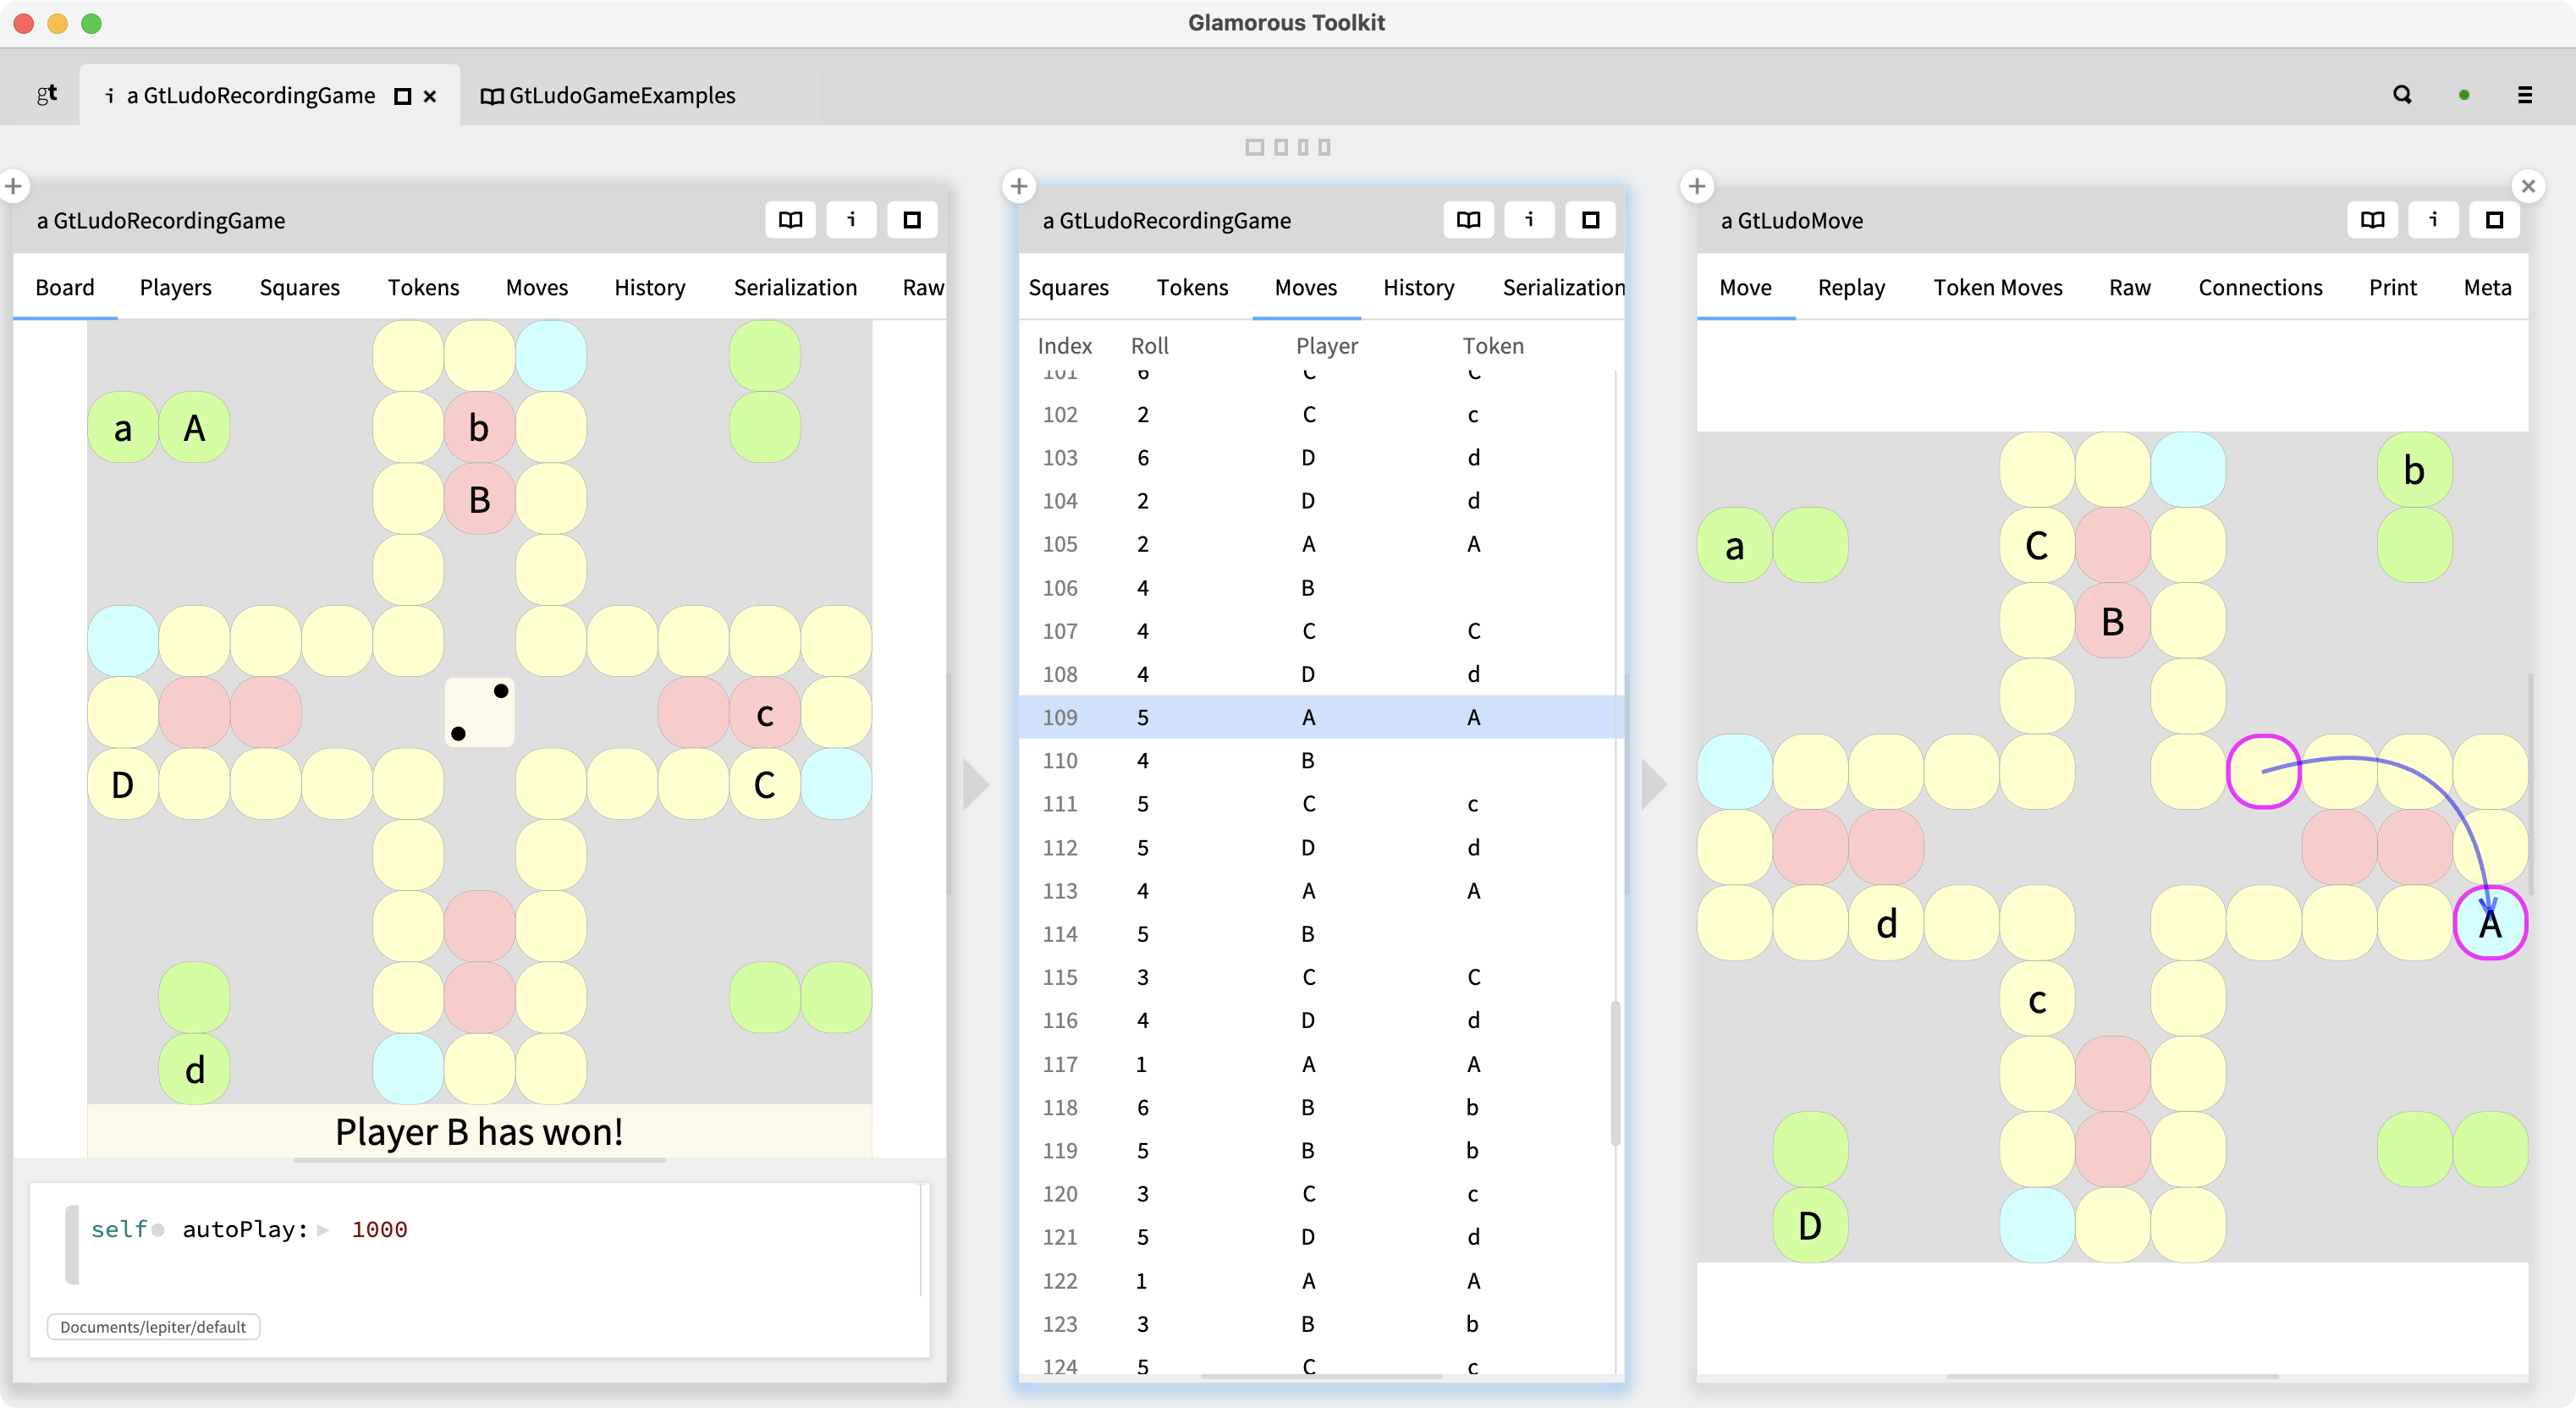
\includegraphics[width=\columnwidth]{custom-views}
  \caption{Custom views of a Ludo game.}
  \label{fig:ludo-views}
\end{figure}

Moldable development is an approach to constructing software systems that are \emph{explainable}.
This is achieved by making it cheap to create dozens, hundreds or even thousands of custom tools to answers questions about a software system, \emph{as these questions arise}.
These custom tools consist of small extensions to the \emph{moldable} tools of the IDE, such as the object inspector, the code browser, the debugger and the notebook.

As a simple example, consider the Inspector views of a Ludo game implementation in \autoref{fig:ludo-views}.
With a conventional implementation, we can either try to play the game interactively, or we can stare at the source code.
We can also run the tests, but if these are all green, they do not help us to understand the system.
By applying moldable development, we turn questions we have about the game into custom views.

The figure shows three connected custom Inspector views of a running game.
In the leftmost pane we see the game GUI as the \st{Board} view.
We can also interact programmatically with the game, evaluating ``\st{self autoPlay: 1000}'' in a contextual playground (a kind of REPL).
In the second pane we can explore the moves of  the completed game, and in the third pane we can explore individual moves.
The \st{Move} view visualizes the actual move performed in the context of the current game state at that point in time.
Each of these views is achieved with just a few lines of code, and leads to the Ludo game becoming an explainable system that can be explored in ways that are far richer and more intuitive than by trying to read source code.

Of course, this begs the question how to actually apply moldable development in practice.
Moldable development is a way to make systems explainable.
This means making the domain model of a software system visible and explorable through custom tools.
This in turn suggests that there are two distinct roles involved in moldable development:
\begin{inparaenum}[(i)]
\item the \emph{Facilitator} is responsible for the technical realization of custom tools, and
\item the \emph{Stakeholder} is responsible for the domain model and questions about the domain that should be answered by the custom tools.
\end{inparaenum}
In a purely technical domain, these two roles can often be played by the same person (\ie a developer), but in general they may be distinct people.


% ===== Moldable Development Patterns =========================
\section{Moldable Development Patterns}

\begin{figure}[h]
  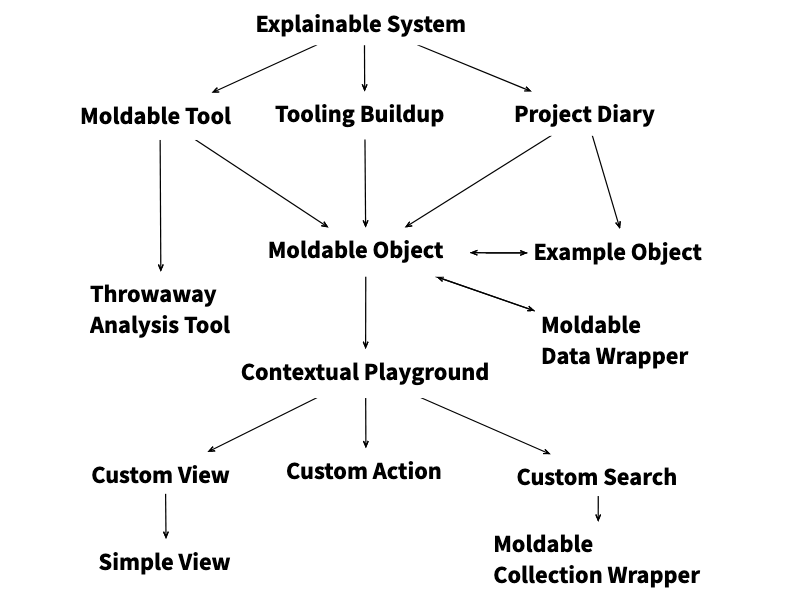
\includegraphics[width=\columnwidth]{map}
  \caption{A map of moldable development patterns.}
  \label{fig:map}
\end{figure}

\on{Do we need all these patterns?}

Moldable development can be understood in terms of a collection of mutually supporting design and process patterns, summarized in \autoref{fig:map}.
These patterns have emerged over several years of experience in developing the Glamorous Toolkit\footnote{\url{https://gtoolkit.com}} moldable development platform, and applying it to numerous systems.
At the root we have the pattern \pattern{explainableSystem}, a software system whose domain model has been exposed with the help of numerous custom tools.
Each custom tool requires the existence of a \pattern{moldableTool}, which can be cheaply adapted with a simple customization.
Some domains require a preliminary phase of \pattern{toolingBuildup}, for example, to create dedicate parsers for programming languages, DSLs or specialized data formats, or bridges to other execution platforms.
A \pattern{projectDiary} is a notebook that serves as a starting point for development tasks.
A \pattern{throwawayAnalysisTool} can be a useful prototype to initially engage a Stakeholder by demonstrating the possibilities of moldable development.

Moldable development itself starts with a \pattern{moldableObject}, a live instance of a domain entity that is explored and molded with custom tools that package the results of exploration tasks.
An interesting instance can be encapsulated as an \pattern{exampleObject}, essentially a unit test that returns a tested object.
An example can be embedded in a project diary notebook page, and can also be used as a moldable object itself for further development tasks.
In case the domain includes already existing data entities, these can be wrapped in a \pattern{viewableDataWrapper} to produce a moldable object.

A moldable object can be explored with the help of its \pattern{contextualPlayground}, a live programming environment bound to the state of a live instance.
Working code can be extracted from such a playground to create custom tools.
The most common of these tools are:
\begin{inparaenum}[(i)]
\item a \pattern{customView}, a dedicated view of an object within a moldable tool such as an object inspector or a code browser, to display or visualize domain-specific information,
\item a \pattern{customAction} that encapsulates a useful domain action, and
\item a \pattern{customSearch}, to perform an ad hoc query over objects reachable from a given moldable object.
\end{inparaenum}
A custom view is frequently a \pattern{simpleView} that can be quickly prototype, and later extended.
A custom search often benefits from a \pattern{collectionWrapper}, to allow the results of a query to be also molded with custom tools.

\on{We have a budget of roughly one column for each pattern. To start with, we keep the patterns to a minimum size. It is easier to expand them than to reduce them in size.}

% ----- Explainable System -------------------------
\subsection*{Explainable System}\label{pat:explainableSystem}

\subsubsection*{Context}

Making technical and non-technical decisions about the further development and evolution of a software system is difficult because the system is complex and hard to understand.

\subsubsection*{Problem}

How can you prepare a software system so that various stakeholders (both technical and non-technical) can easily answer questions they have about it?

\subsubsection*{Forces}

Source code is impossible to read at scale.
Static documentation tends to get out of date.
The live, running system is designed to fulfil end user use cases, not answering technical or business questions.
Generic analysis tools and IDEs are unlikely to be able to answer domain-specific questions about your system.
Developing custom tools can be costly and time-consuming.

\subsubsection*{Solution}

Transform the software system into a ``live'' domain model in which each domain entity can be interactively explored with the help of custom tools, \ie simple views and visualizations, metrics, queries, and operations.
Leverage open, ``moldable'' IDE tools to reduce the cost of building custom tools.
Drive the development of the custom tools by concrete questions you have about the system.

\on{Add pointers to some subsequent patterns.}

\subsubsection*{Consequences}

The custom tools become part of the live, running system.
Unlike static documentation, the custom tools are more likely to stay in sync with the evolving system.
\on{More ... Also some negative consequences?}

% ----- Moldable Tool -------------------------
\subsection*{Moldable Tool}\label{pat:moldableTool}

\subsubsection*{Context}
\subsubsection*{Problem}
\subsubsection*{Forces}

\subsubsection*{Solution}

Make the IDE tools moldable by making it easy to plug in new behavior.
\on{Add citation ...}\cite{Chis17a}


\subsubsection*{Consequences}



% ----- Tooling Buildup -------------------------
\subsection*{Tooling Buildup}\label{pat:toolingBuildup}
\subsubsection*{Context}
\subsubsection*{Problem}
\subsubsection*{Forces}
\subsubsection*{Solution}
\subsubsection*{Consequences}



% ----- Throwaway Analysis Tool -------------------------
\subsection*{Throwaway Analysis Tool}\label{pat:throwawayAnalysisTool}
\subsubsection*{Context}
\subsubsection*{Problem}
\subsubsection*{Forces}
\subsubsection*{Solution}
\subsubsection*{Consequences}


% ----- Project Diary -------------------------
\subsection*{Project Diary}\label{pat:projectDiary}
\subsubsection*{Context}
\subsubsection*{Problem}
\subsubsection*{Forces}
\subsubsection*{Solution}
\subsubsection*{Consequences}


% ----- Moldable Object -------------------------
\subsection*{Moldable Object}\label{pat:moldableObject}
\subsubsection*{Context}
\subsubsection*{Problem}
\subsubsection*{Forces}
\subsubsection*{Solution}
\subsubsection*{Consequences}

% ----- Example Object -------------------------
\subsection*{Example Object}\label{pat:exampleObject}
\subsubsection*{Context}
\subsubsection*{Problem}
\subsubsection*{Forces}
\subsubsection*{Solution}
\subsubsection*{Consequences}

% ----- Viewable Data Wrapper -------------------------
\subsection*{Viewable Data Wrapper}\label{pat:viewableDataWrapper}
\subsubsection*{Context}
\subsubsection*{Problem}
\subsubsection*{Forces}
\subsubsection*{Solution}
\subsubsection*{Consequences}


% ----- Contextual Playground -------------------------
\subsection*{Contextual Playground}\label{pat:contextualPlayground}
\subsubsection*{Context}
\subsubsection*{Problem}
\subsubsection*{Forces}
\subsubsection*{Solution}
\subsubsection*{Consequences}


% ----- Custom View -------------------------
\subsection*{Custom View}\label{pat:customView}
% AKA Viewable Entity
\subsubsection*{Context}
\subsubsection*{Problem}
\subsubsection*{Forces}
\subsubsection*{Solution}
\subsubsection*{Consequences}



% ----- Simple View -------------------------
\subsection*{Simple View}\label{pat:simpleView}
\subsubsection*{Context}
\subsubsection*{Problem}
\subsubsection*{Forces}
\subsubsection*{Solution}
\subsubsection*{Consequences}



% ----- Custom Action -------------------------
\subsection*{Custom Action}\label{pat:customAction}
\subsubsection*{Context}
\subsubsection*{Problem}
\subsubsection*{Forces}
\subsubsection*{Solution}
\subsubsection*{Consequences}


% ----- Custom Search -------------------------
\subsection*{Custom Search}\label{pat:customSearch}
\subsubsection*{Context}
\subsubsection*{Problem}
\subsubsection*{Forces}
\subsubsection*{Solution}
\subsubsection*{Consequences}


% ----- Collection Wrapper -------------------------
\subsection*{Collection Wrapper}\label{pat:collectionWrapper}
\subsubsection*{Context}
\subsubsection*{Problem}
\subsubsection*{Forces}
\subsubsection*{Solution}
\subsubsection*{Consequences}


%% The next two lines define the bibliography style to be used, and
%% the bibliography file.
\bibliographystyle{ACM-Reference-Format}
\bibliography{moldablePatterns}


\end{document}
\endinput

% ===== TEMPLATES =========================

% ----- PATTERN -------------------------
\subsection*{PATTERN}\label{pat:PATTERN}
\subsubsection*{Context}
\subsubsection*{Problem}
\subsubsection*{Forces}
\subsubsection*{Solution}
\subsubsection*{Consequences}


\begin{inparaenum}[(i)]
\item
\item
\end{inparaenum}

